%----------------------------------------------------------------------------
\section{Ábrák és táblázatok}
%----------------------------------------------------------------------------
A képeket PDFLaTeX esetén a veszteségmentes PNG, valamint a veszteséges JPEG formátumban érdemes elmenteni. Az EPS (PostScript) vektorgrafikus képformátum beillesztését a PDFLatex közvetlenül nem támogatja. Ehelyett egy lehetőség 200 dpi, vagy annál nagyobb felbontásban raszterizálni a képet, és PNG formátumban elmenteni. Az egyes képek mérete általában nem, de sok kép esetén a dokumentum összmérete így már szignifikáns is lehet. A dokumentumban felhasznált képfájlokat a dokumentum forrása mellett érdemes tartani, archiválni, mivel ezek hiányában a dokumentum nem fordul újra. Ha lehet, a vektorgrafikus képeket vektorgrafikus formátumban is érdemes elmenteni az újrafelhasználhatóság (az átszerkeszthetőség) érdekében.

Kapcsolási rajzok legtöbbször kimásolhatók egy vektorgrafikus programba (pl. CorelDraw) és onnan nagyobb felbontással raszterizálva kimenthatők PNG formátumban. Ugyanakkor kiváló ábrák készíthetők Microsoft Visio vagy hasonló program használatával is: Visio-ból az ábrák közvetlenül PNG-be is menthetők.

Lehetőségeink Matlab ábrák esetén:
\begin{itemize}
	\item Képernyőlopás (\emph{screenshot}) is elfogadható minőségű lehet a dokumentumban, de általában jobb felbontást is el lehet érni más módszerrel.
	\item A Matlab ábrát a \verb+File/Save As+ opcióval lementhetjük PNG formátumban (ugyanaz itt is érvényes, mint korábban, ezért nem javasoljuk).
	\item A Matlab ábrát az \verb+Edit/Copy figure+ opcióval kimásolhatjuk egy vektorgrafikus programba is és onnan nagyobb felbontással raszterizálva kimenthatjük PNG formátumban (nem javasolt).
	\item Javasolt megoldás: az ábrát a \verb+File/Save As+ opcióval EPS \emph{vektorgrafikus} formátumban elmentjük, PDF-be konvertálva beillesztjük a dolgozatba.
\end{itemize}
Az EPS kép az \verb+epstopdf+ programmal\footnote{a korábban említett \LaTeX-disztribúciókban megtalálható} konvertálható PDF formátumba. Célszerű egy batch-fájlt készíteni az összes EPS ábra lefordítására az alábbi módon (ez Windows alatt működik).
\begin{lstlisting}[frame=single,float=!ht]
@echo off
for %%j in (*.eps) do (
echo converting file "%%j"
epstopdf "%%j"
)
echo done .
\end{lstlisting}

Egy ilyen parancsfájlt (\verb+convert.cmd+) elhelyeztük a sablon \verb+figures\eps+ könyvtárába, így a felhasználónak csak annyi a dolga, hogy a \verb+figures\eps+ könyvtárba kimenti az EPS formátumú vektorgrafikus képet, majd lefuttatja a \verb+convert.cmd+ parancsfájlt, ami PDF-be konvertálja az EPS fájlt.

Ezek után a PDF-ábrát ugyanúgy lehet a dokumentumba beilleszteni, mint a PNG-t vagy a JPEG-et. A megoldás előnye, hogy a lefordított dokumentumban is vektorgrafikusan tárolódik az ábra, így a mérete jóval kisebb, mintha raszterizáltuk volna beillesztés előtt. Ez a módszer minden -- az EPS formátumot ismerő -- vektorgrafikus program (pl. CorelDraw) esetén is használható.

A képek beillesztésére az \sectref{LatexTools}. fejezetben mutattunk be példát (\figref{TexnicCenter}~ábra). Az előző mondatban egyúttal az automatikusan feloldódó ábrahivatkozásra is láthatunk példát. Több képfájlt is beilleszthetünk egyetlen ábrába. Az egyes képek közötti horizontális és vertikális margót metrikusan szabályozhatjuk (\figref{HVSpaces}~ábra). Az ábrák elhelyezését számtalan tipográfiai szabály egyidejű teljesítésével a fordító maga végzi, a dokumentum írója csak preferenciáit jelezheti a fordító felé (olykor ez bosszúságot is okozhat, ilyenkor pl. a kép méretével lehet játszani).

\begin{figure}[!ht]
\centering
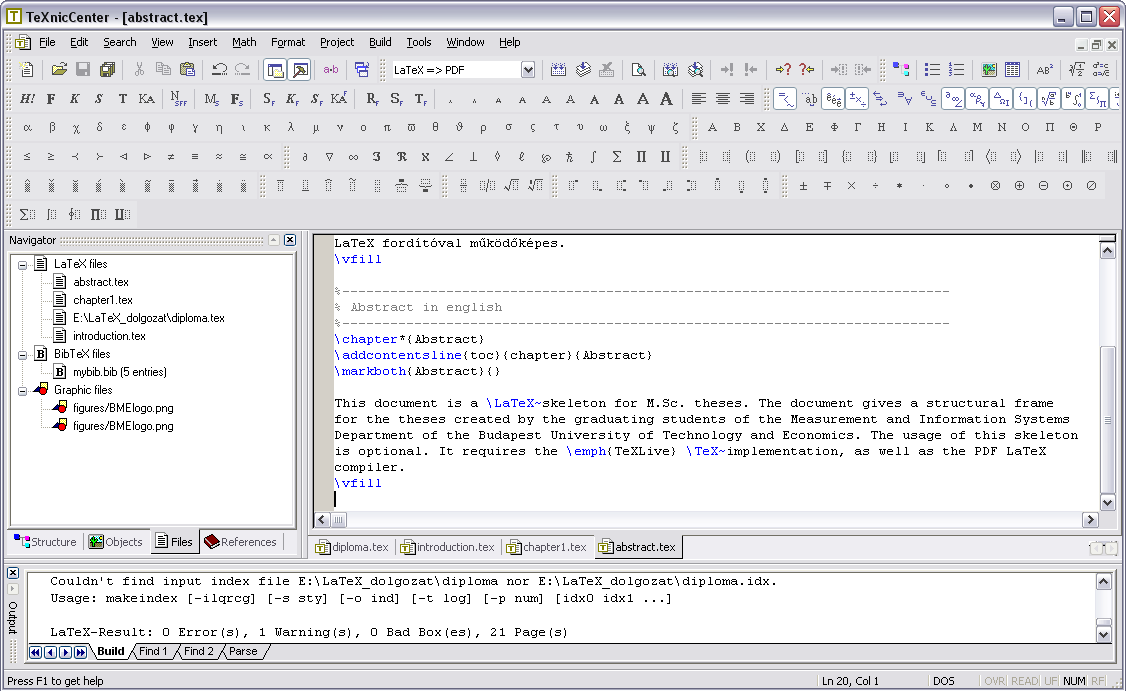
\includegraphics[width=67mm, keepaspectratio]{figures/TeXnicCenter.png}\hspace{1cm}
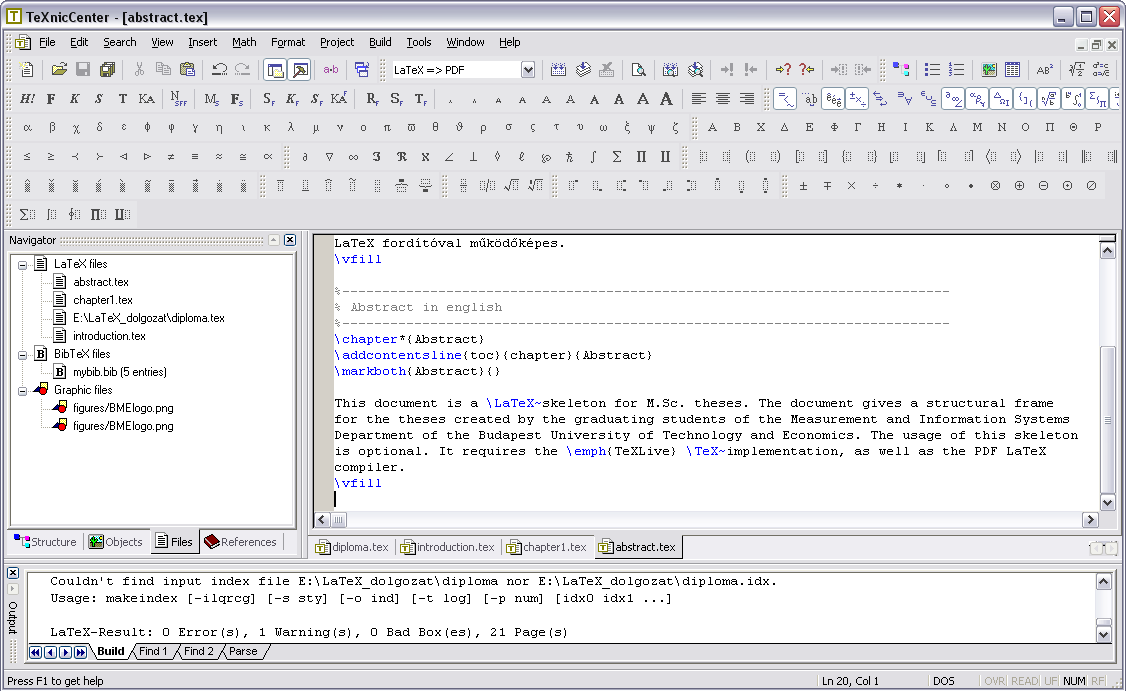
\includegraphics[width=67mm, keepaspectratio]{figures/TeXnicCenter.png}\\\vspace{5mm}
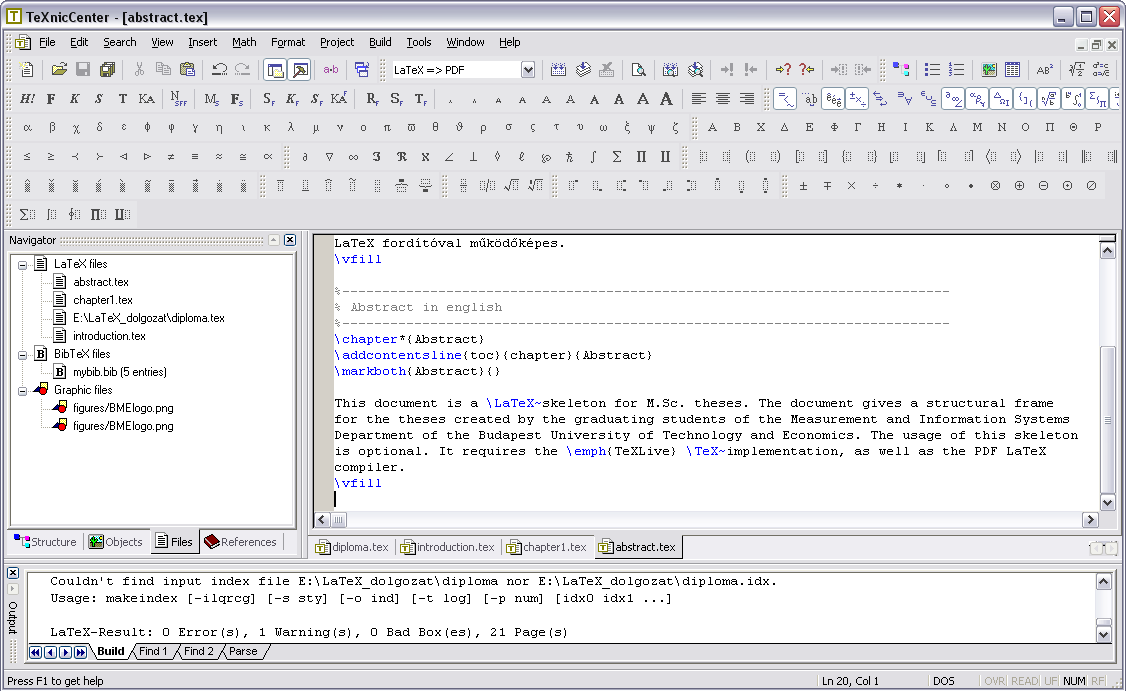
\includegraphics[width=67mm, keepaspectratio]{figures/TeXnicCenter.png}\hspace{1cm}
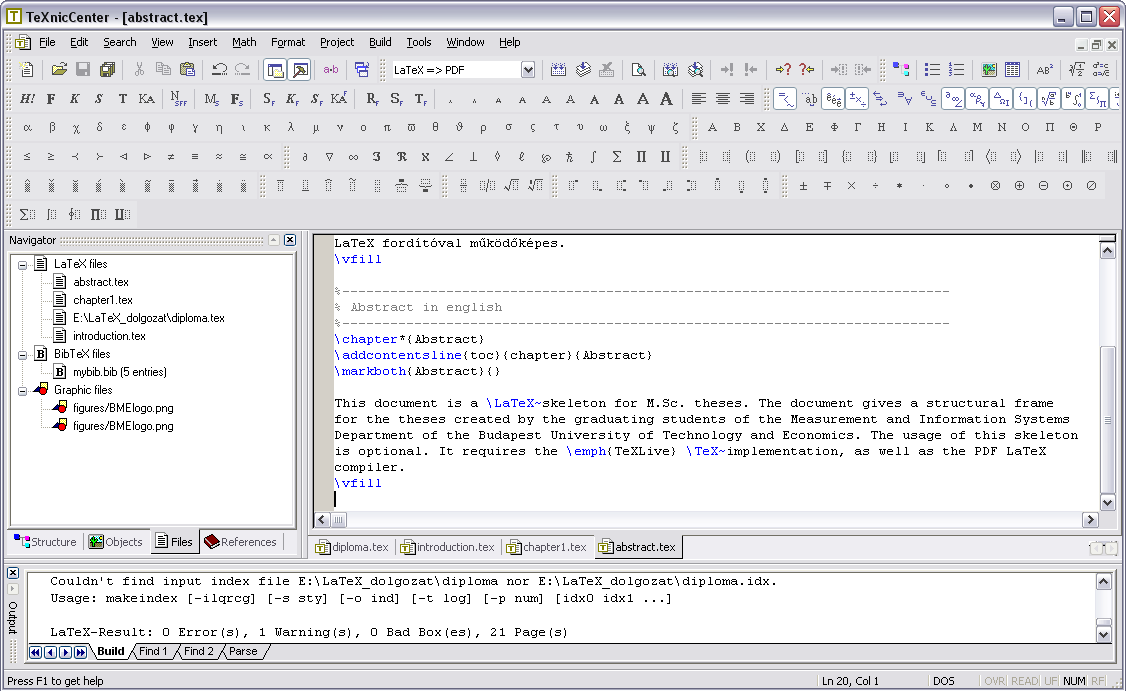
\includegraphics[width=67mm, keepaspectratio]{figures/TeXnicCenter.png}
\caption{Több képfájl beillesztése esetén térközöket is érdemes használni.} 
\label{fig:HVSpaces}
\end{figure}

A táblázatok használatára a \tabref{TabularExample}~táblázat mutat példát.
A táblázat címkéje nem véletlenül került a táblázat fölé, ez a szokványos.
\begin{table}[ht]
	\footnotesize
	\centering
	\caption{Az órajel-generátor chip órajel-kimenetei.} \label{tab:SysClocks}
	\begin{tabular}{ | l | c | c |}
	\hline
	Órajel & Frekvencia & Cél pin \\ \hline
	CLKA & 100 MHz & FPGA CLK0\\
	CLKB & 48 MHz  & FPGA CLK1\\
	CLKC & 20 MHz  & Processzor\\
	CLKD & 25 MHz  & Ethernet chip \\
	CLKE & 72 MHz  & FPGA CLK2\\
	XBUF & 20 MHz  & FPGA CLK3\\
	\hline
	\end{tabular}
	\label{tab:TabularExample}
\end{table}
